\section{Quality of Service}

Traffic prioritization, resource reservation control mechanisms, guarantees for certain levels of performance, etc. Important for real-time / inelastic applications (streaming, gaming, voIP, critical / safety-related, etc.). IP network = best-effort network which does not support QoS.

How to configure a router to manage congestion. See Figure \ref{fig:qos} for an overview of the components.

\begin{figure}[h]
	\centering
	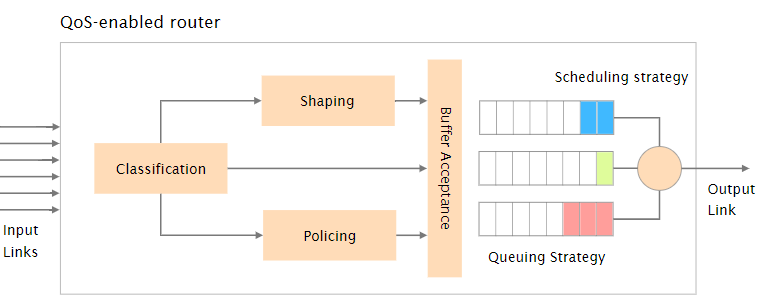
\includegraphics[scale=0.7]{images/2-qos.PNG}
	\caption{Components of a QoS enabled router.}
	\label{fig:qos}
\end{figure}

\subsection{Scheduling / Queuing Strategy}

%TODO more algos?

\paragraph{Scheduling}
Which buffered packets get send out next and when? Either work-conserving (link is never idle) or non-work conserving. Also, algorithms that maintain per-flow state typically do not scale. In practice, policies are combined to accommodate a number of classes of traffic.

\paragraph{FIFO} The first packet that arrives is the first one that leaves. Simple and no starvation but does not allow for prioritization and can be unfair.

\paragraph{Priority Queue}
Higher priority queues always get serviced first. Packets are classified. For each queue, packets serviced in a FIFO manner. Simple, allows for differentiation and isolating high priority traffic but starvation is a risk.

\paragraph{(Weighted) Fair Queue}
One queue per flow, round-robin to service all queues. Divide bandwidth among all flows equally. Weighted (fraction) allows for bandwidth allocation to each flow (not equal). Provides isolation and fairness (approximates max-min fair allocation, perfect if all packets have equal size - if not, smaller packets get penalized), but is very demanding resource-wise (one queue per flow) and thus doesn't scale. Perfect would be bit-by-bit queuing but way too complex and impossible. 

WFQ = FQ if weight for each queue is 1 over number of flows.
%TODO bit-by-bit approximation thingy

\paragraph{Max-Min Fairness}
Given a set of bandwidth demands $b_i$ and a total bandwidth $C$, the max-min bandwidth allocations $a_i$ are:

$$a_i = \text{min}(f, b_i)$$

where $f$ is the unique value (fair share) s.t. $\Sigma a_i = C$. This means that if a flow doesn't get full demand, no other flow gets more than the flow. Intuition: water filling different-capacity pipes, continue filling until no more water or all pipes full.

\begin{figure}[h]
	\centering
	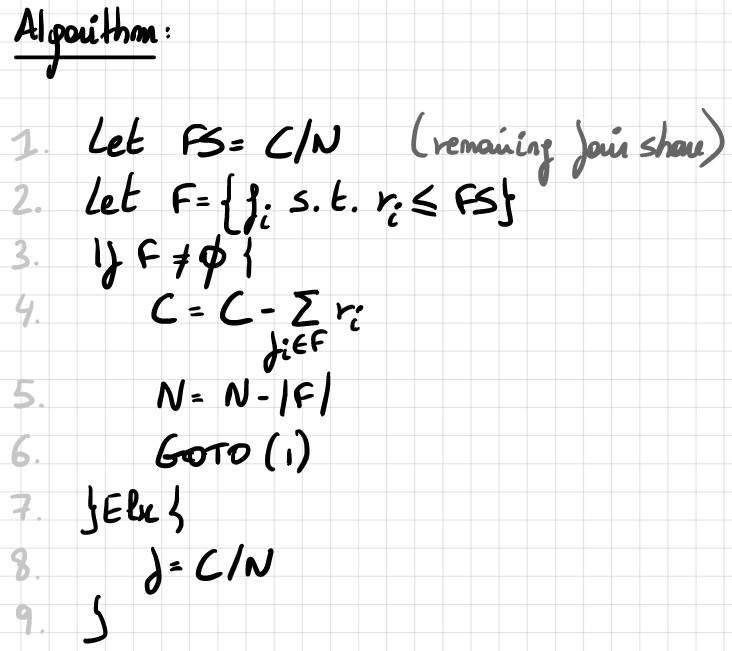
\includegraphics[scale=0.5]{images/2-maxmin.PNG}
	\caption{Computing Max-Min Fairness.}
	\label{fig:maxmin}
\end{figure}

%TODO algo example

\subsection{Buffer Acceptance}

After knowing which queue to append a packet to, router needs to decide whether to accept or drop it. By dropping packets, we signal to the sender to lower its rate (congestion).

\paragraph{Tail Drop}
Simply drop any newly arriving packets when the queue is full. Con: synchronizes TCP flows when multiple packets are lost (all sources backtrack the same). Also, it's completely agnostic.

\paragraph{Random Early Detection (RED)}
Instead of dropping when full, start dropping early as a preventive measure. The fuller the buffer, the more likely a packet is dropped. You're more likely to be dropped if you're causing the congestion. Randomness avoids global synchronization.

\begin{figure}[h]
	\centering
	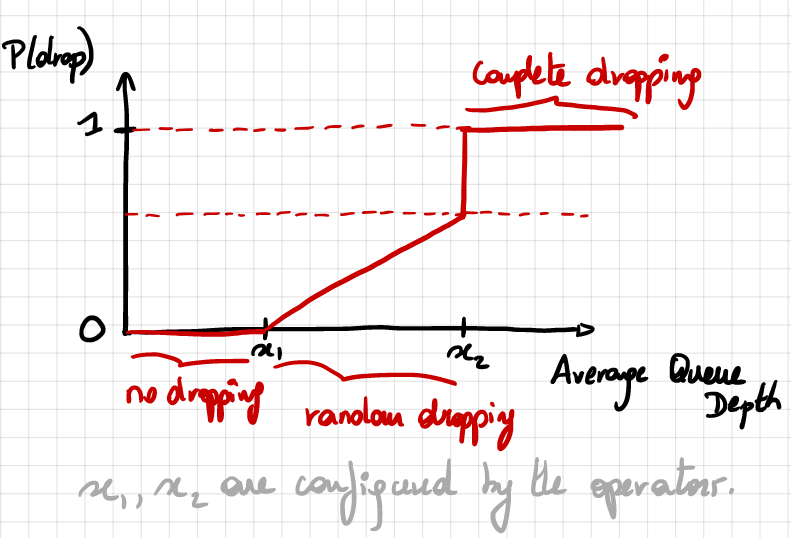
\includegraphics[scale=0.5]{images/2-red.PNG}
	\caption{RED visualized.}
	\label{fig:red}
\end{figure}

\subsection{Shaping and Policing}

\paragraph{Shaping}
Regulating the traffic by changing the outgoing rate.

\paragraph{Policing}
Specifying rules such as "only use x Gbps" and drop everything going over it.

\paragraph{Specifying Rates}
How to unambiguously characterize / monitor the throughput requirement of an application? By specifying / monitoring the burstiness of traffic (average rate and burst size) we can deal with both the max. rate and not be wasteful (don't just look at max or average).

\paragraph{Token Bucket Algorithm}
Used to check that sending rate conforms to defined limits on bandwidth and burstiness or can also be used as a scheduling algorithm.

Bucket with a fixed capacity filled with tokens representing units / bytes at a fixed rate. Every packet is checked by inspecting the bucket to see if it contains sufficient tokens at that time. If so, appropriate number of tokens is removed and packet is sent.

Conforming flows can contain traffic with average rate equal to bucket filling rate and burstiness determined by depth of bucket.

\begin{figure}[h]
	\centering
	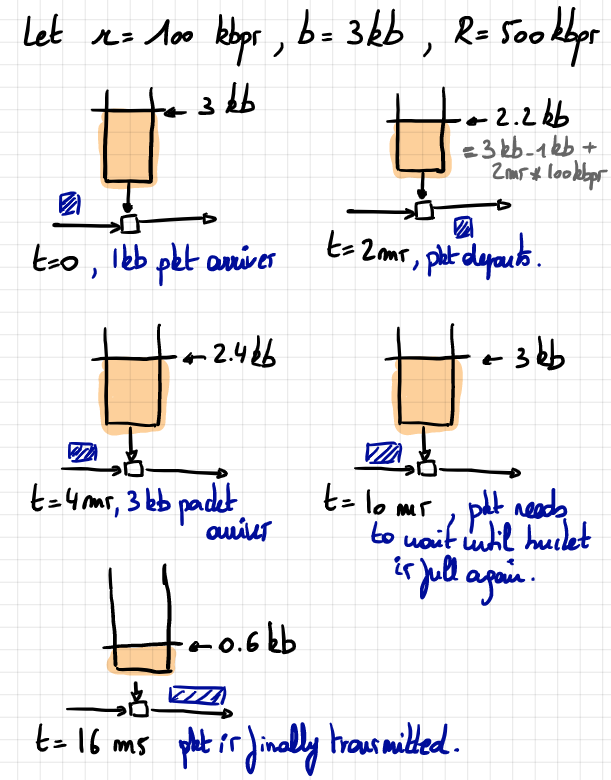
\includegraphics[scale=0.5]{images/2-bucketexample.PNG}
	\caption{Token Bucket example (filling rate, bucket depth and output rate).}
	\label{fig:bucket}
\end{figure}

\textbf{Non-Compliant Packets:} In the example, the non-compliant packet is delayed until it becomes compliant (shaping). One can also drop it (policing) or mark it (marking) which  gives the packet a lower priority. These are three things one can use a token bucket for.


%TODO lec 7 TB scheduling, classification what does it say

\subsection{Classification}

To enqueue packets in different queues with varying priorities, we need a way to classify them. For example, all TCP traffic is one class and all SSH traffic another. Or, customers are their own class. Anything can be a predicate to classify traffic and mark it accordingly.